\chapter{GPS Concept and Error Sources}

Along with earlier navigation systems, this chapter explains the positioning concept of GPS and modern Global Navigation Satellite Systems in general.
The error sources that impact the accuracy of GPS are listed and split into categories that determine in which segment those errors occur.


\section{Predecessors}
Before there was GPS, other radionavigation systems were used.
They were mostly ground based and limited to a certan area or time.

One of the early examples is the U.S. system \textit{Loran}.
It works with multiple transmission stations with a distance of about 1000km to each other.
They send out pulse signals in all directions.
With the difference in time-of-arrival of those pulses, a receiver can triangulate its position.
This method is one variant of hyperbolic positioning.
Only a 2D fix can be acieved with such systems.
The height, if needed, has so be determined with a different method.
The development of \textit{Loran-A} was started during World War \rom{2}.
\textit{Loran-C} is the latest version and still in use today
It has a rms positioning accuracy of about 250m.

Another hyperpolic positioning system was \textit{Omega}.
It was the first global radionavigation system and operational from 1970 to 1997.
But rather than measuring the time differene of pulses, the phase difference of sinusoidal signals was measured.
This method resulted in a rms postitoning accuracy of 2-4km.
The lower accuracy can be explained with the much wider area it had to cover.

Apart from those ground based systems, there was a working satellite navigation system that came even before \textit{Omega}.
It is called \textit{Transit} and was operational from 1964 to 1996.
A doppler based systen that was launched by the U.S. Navy.
In doppler positioning, a 2D position can be determined from the time the doppler of the satellite signal changes from high to low and the sharpnes of the change.
At the moment the doppler changes, the satellite is the closest to the receiver on its orbit.
The distance from the projected orbit can then be determined by how sharp the doppler changes.
When the receiver is directly on the projected orbit, the doppler changes the fastest.
In contrast to modern GNSS, \textit{Transit} satellites had polar orbits with a low altitude of 1100km.
Only one satellite was visible at a time with a wait time of up to 100 minutes between them.
This made positioning a relatively long process, but the rms positioning accuracy was much better with 25m.

A range of counterparts from Russia and Eurpoe existed to those U.S. systems.
\textit{Gee} was a hyperbolic system from Great Britain similar to Loran.
It was used by the Royal Air Force during World War \rom{2}.
Doppler positioning was already used in reverse to determine the orbit of \textit{Sputnik \rom{1}} from a ground station with a known location.
The idea to measure the postiton on earth came from this application.
The Soviet Union had two dopple based system similar to \textit{Transit} called \textit{Parus} and \textit{Tsikada}. \cite{misra2011global}


\section{Global Navigation Satellite Systems}

From the knowledege gained from \textit{Tansit}, a new class of space based navigation systems emerged. 
The first one beeing the NAVSTAR Global Positioning System (GPS) developed by the U.S. Government.
The first GPS satellite was launched in 1978 and the system became fully operantional in 1993.
To be independent from the U.S. when it comes to navigation and improve local positioning, other nations started to launch their own systems.
The generic term for such systems is Global Navigation Satellite Systems (GNSS).
The fisrt addition to the group was the former Soviet and now Russian system GLONASS.
It is very similar to GPS in terms of use case and architecture.
Both were mainly developed for military use and designed to cover the whole globe with a full constellation of 24 satellites in medium earth orbit. \cite{misra2011global}

A newer addition is the european system GALILEO.
It is similar in terms of system architecture to GPS and GLONASS, but it is the first GNSS that is under civilian controll.
This guarantees that civil receivers can get the highest precission possible.
The GALILEO constellation is not yet complete with 14 usable satellites at the moment, but it is said to improve the accuracy to the centimeter level in normal operation. \cite{GSA_Galileo}

Beside global navigation systems, there are also local programs which improve the regional accuracy.
They consist of satellites in geostationary or geosynchronous orbits.
This gives them a constant location above the earth or within a few degreees of longitude.
Such systems are the Japanese QZSS and the Indian IRNSS.
The Chinese BeiDou system is a combination of global and regional.
It started with just geostationary and geosynchronous satellites over China, but now has three operational global satellites with more to come.


\section{GPS}

This section explains the 

\subsection{Functional Principle}

All modern GNSS work with the principle of trilateration.
For this method of postitoning, the distance to three known lacations is needed to calculate the own position in three dimensions.
With radio waves, the distance to a transmitting station can be measured trough the propagation time of the wave.
The distance is calculated when the propagation speed is divided by the propagation time.
Ground based systems can only solve for the position on a two dimensional plane because they are limited in transmitter height above the surface of the earth.
A space-based system can also solve for height with transmitters distributed in all three dimensions.

This is achieved with satellites as transmission stations.
GPS satellites are in medium earth orbit at an altitude of about 20'200km with each satellite circling the earth twice a day.
The orbits of GLONASS are a bit lower and GALILEO a bit higher.

\begin{figure}[ht]
 \centering
 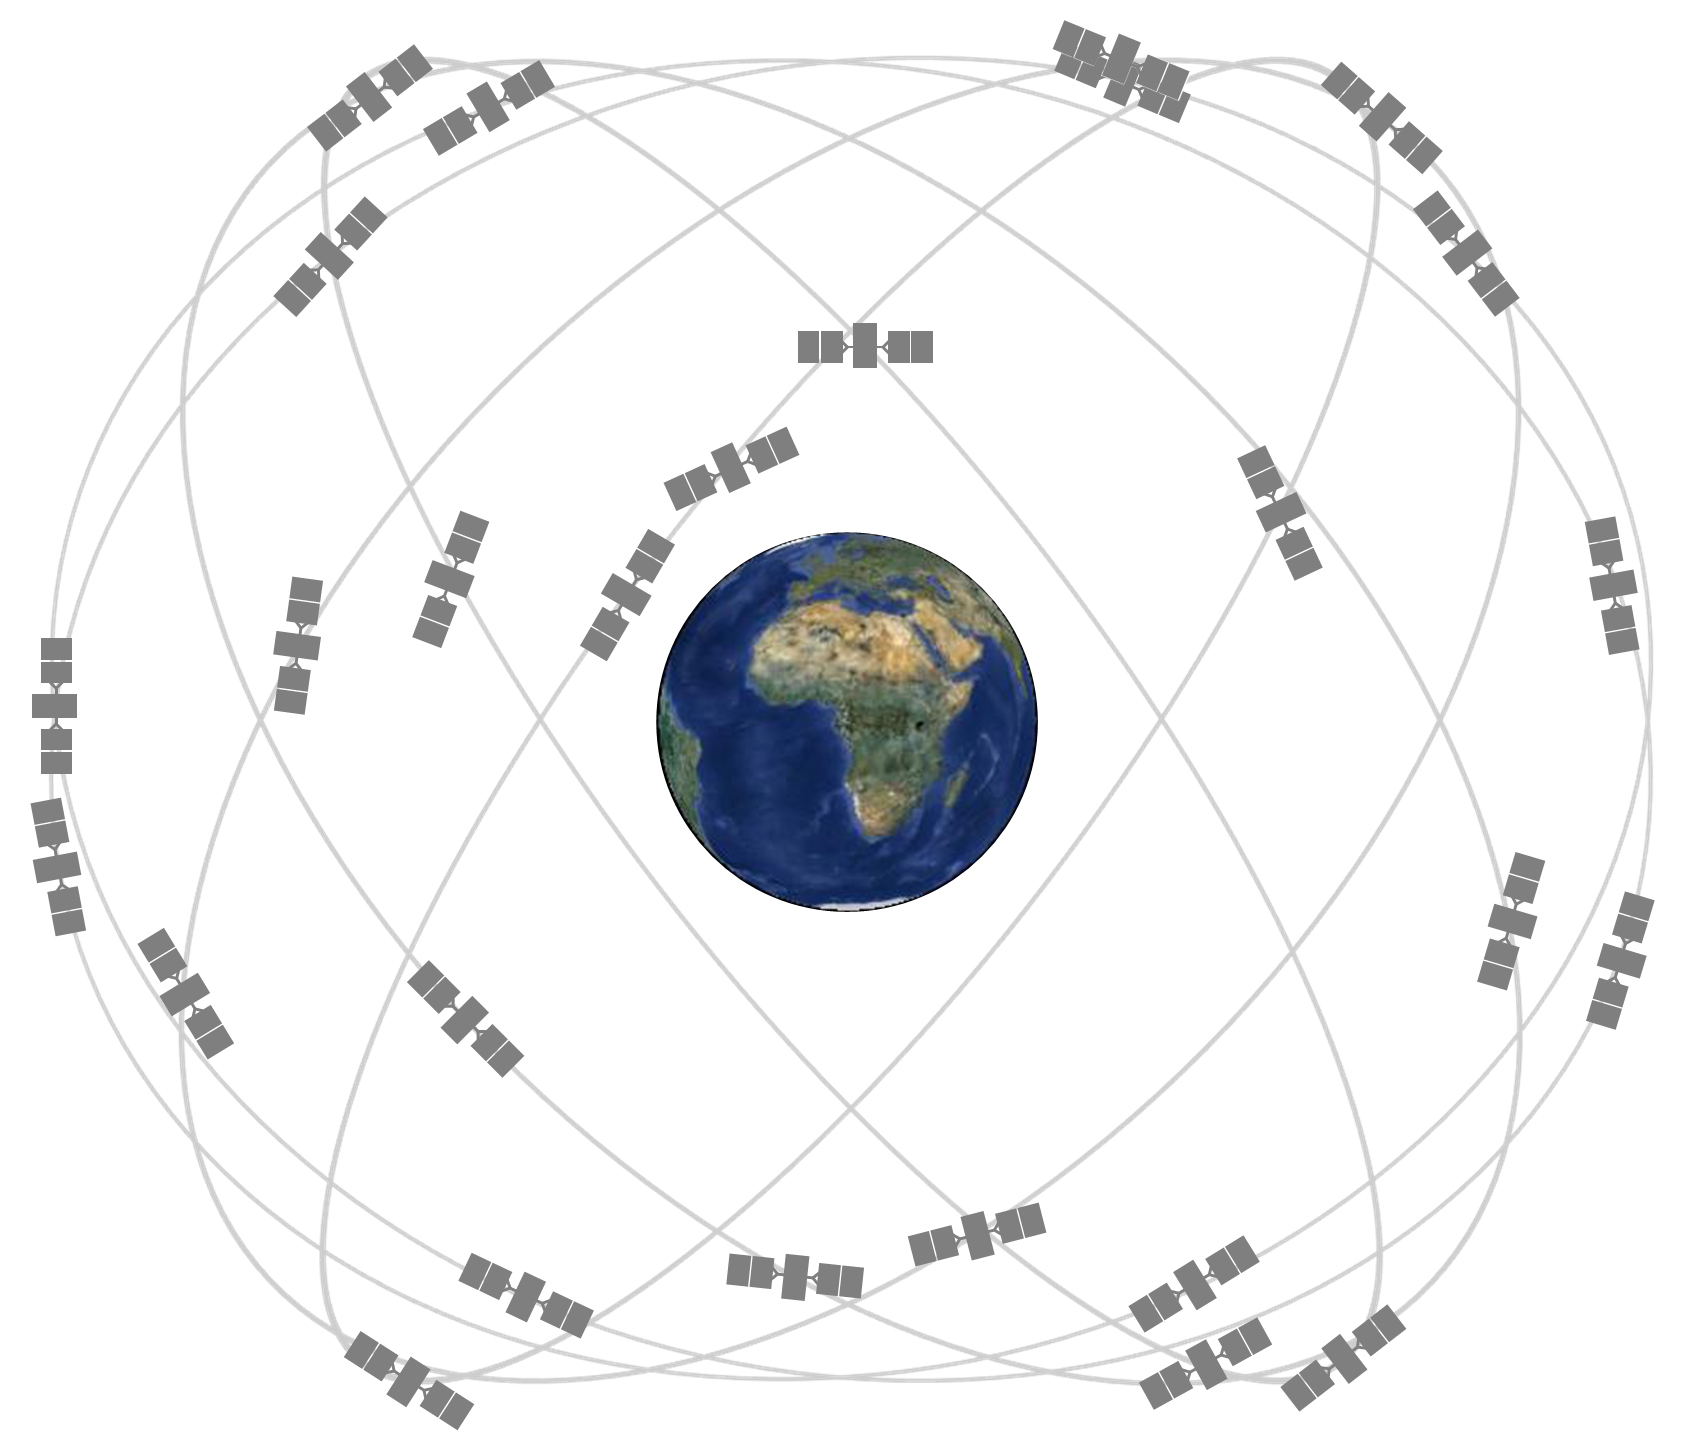
\includegraphics[height=5cm]{images/constellation.jpg}
 \caption{GPS satellite constellation \cite{GPS_GOV}}
\end{figure}


 
\subsection{Signals}

\subsection{Performance}


\section{Error Sources}

\subsection{Satellite Errors}

\subsection{Signal Propagation Errors}

\subsection{Receiver Errors}
